\section{Conservation Laws}
% What is a fluid?
The Conservation Laws are the fundamental physical principles that describe the nature's observable behavior of mass continuity, momentum and energy conservation. Given a finite volume in space assumed as a continuum domain where only macroscopic properties are sufficient to describe its behavior, the conservation laws formulate that the total variation of a conservative quantity in a unit time is equivalent of the total amount of this quantity that flows across the volume's surfaces plus any external source. This principle can be written in differential form as

\begin{equation}  \label{eq:eq_cons}
\frac{\partial \textbf{Q}}{\partial t} = -\nabla \cdot \textbf{F} + \textbf{S}
\mbox{ .}
\end{equation}
where $\textbf{Q}$ represents the fluid macroscopic quantities such as mass, momentum and total energy per unit of volume, and $\textbf{F}$ the flux of these quantities that passes across the volume's surfaces, and $\textbf{S}$ the source or sink term per unit of volume.

\section{Euler Equations}
% What? Why? How? Where?
The Euler equations are the mathematical formulation that model compressible, non-heat-conducting, inviscid flows composed by the conservation laws of mass, momentum and total energy. The physical phenomena represented by the Euler equations are, hence, fluid flows on the edge of almost zero viscosity where the convective effects are dominant. These equations can be expressed in several forms, nevertheless, in the presence of physical discontinuities such as contact and shock waves, it is recommended the use of the conservation form to correctly compute the intensity and propagation speed of these waves \cite{Hirsch1991}. The system of the 2-D Euler equations in the conservative form, in the absence of source terms, can be written as
% Ref.: Vol. 2 Hirsch Pag. 132
%
\begin{equation} \label{eq:eq_euler}
    \frac{\partial \textbf{Q}}{\partial t} + \frac{\partial \textbf{F}}{\partial x} + \frac{\partial \textbf{G}}{\partial y} = 0
    \mbox{ .}
\end{equation}
%
where $\textbf{Q}$ is the vector of conserved variables, $\textbf{F}$ and $\textbf{G}$ the inviscid flux vectors for x and y directions, given by 
%
\begin{equation}
    \label{eq:eq_euler_defs}
    \textbf{Q} = \left\{ \begin{array}{c} \rho \\ \rho u \\ \rho v \\ E
    \end{array} \right\} \mbox{ ,} \hspace*{1.0 cm}
    \textbf{F} = \left\{ \begin{array}{c} \rho u \\ \rho u^2 + p \\ \rho uv \\ u(E + p)
    \end{array} \right\} \mbox{ ,} \hspace*{1.0 cm}
    \textbf{G} = \left\{ \begin{array}{c} \rho v \\ \rho uv \\ \rho v^2 + p \\ v(E + p)
    \end{array} \right\} \mbox{ .}
\end{equation}
%
forming a hyperbolic system of first-order partial differential equations. The $\rho$ is the density, $p$ is the pressure, $E$ is the total energy, $u$ and $v$ the velocity components in x and y directions, respectively, representing the set of primitive variables. In order to form a closed system of equations, an additional relation between the pressure and the other primitive variables is defined from the equation of state for perfect gases as
%
\begin{equation}
    \label{eq:eq_gases}
    p = (\gamma-1) \left[ E - \frac{1}{2}\rho(u^2+v^2) \right]
\end{equation}
%
where $\gamma$ is the isentropic exponent.
% Ideal Gas assumption impacts
Equation\ \eqref{eq:eq_gases} can be derived by the assumption of negligible intermolecular forces in the ideal gas law, $p = \rho RT$, where $T$ is the fluid temperature and $R$ the specific gas constant. The assumptions behind the ideal gas law are only valid when the gas particles have negligible volume, have perfect elastic collisions with no energy loss, particles are equally sized and no intermolecular forces are presented. Additionally, the fluid is also assumed to be thermally and calorically perfect, i.e., the fluid internal energy, $e$, and enthalpy, $H$, are only functions of the temperature and the specific heat capacity at constant volume, $c_v$, and pressure, $c_p$, are constants. Specific enthalpy, $h$, and internal energy per unit of mass can then be obtained from
%
\begin{align*}
    \label{eq:eq_tps}
    e &= c_vT  & h &= \frac{H}{\rho} = c_pT
\end{align*}
%

By the definition of enthalpy 
%
\begin{equation}
    \label{eq:eq_enthalpy}
	h = e + \frac{p}{\rho}
\end{equation}
%
and Eq.\ \eqref{eq:eq_gases}, a relation between the specific heat capacity can be obtained
%
\begin{equation}
    \label{eq:eq_heats}
    c_p - c_v = R
\end{equation}
%
which can be solved for each specific heat capacity coefficients by defining the ratio of specific heat capacities as
%
\begin{equation}
    \label{eq:eq_heats2}
    \gamma = \frac{c_p}{c_v}
\end{equation}
%
leading to the expressions
%
\begin{align}
    \label{eq:eq_heats3}
    c_p &= \frac{\gamma R}{\gamma-1}      &     c_v &= \frac{R}{\gamma-1}
\end{align}

\section{Formulation of Characteristic Equations}
The flux vector of the Euler equations can be rewritten as a function of the fluid conservative properties from the $\textbf{Q}$ vector components
%
\begin{align}
    \label{eq:euler_sol_vec}
    \textbf{Q} &= \left\{ \begin{array}{c} \rho \\ \rho u \\ \rho v \\ E
    \end{array} \right\} = \left\{ \begin{array}{c} q_1 \\ q_2 \\ q_3 \\ q_4
    \end{array} \right\}
\end{align}    
%
so that the flux vectors become
%
\begin{align}
    \label{eq:euler_flx_vec}
    \textbf{F} &= \left\{ \begin{array}{c} 
    	q_2 \\ 
	    \frac{{q_2}^{2}}{q_1} + p \\
	    \frac{q_2 q_3}{q_1} \\
	    \frac{q_2}{q_1}\left( q_4 + p \right)
    \end{array} \right\} &
    \textbf{G} &= \left\{ \begin{array}{c} 
    	q_3 \\ 
    	\frac{q_3}{q_1} q_2 \\
    	\frac{{q_3}^{2}}{q_1} + p \\    	 
    	\frac{q_3}{q_1}\left( q_4 + p \right)
    \end{array} \right\}    
\end{align}
%
where the pressure $p$ can also be represented by the $\textbf{Q}$ components as
%
\begin{equation}
    \label{eq:eq_pressure}
    p = (\gamma-1)\left[ q_4 - \frac{({q_2}^2 + {q_3}^2)}{2 q_1} \right]
\end{equation}
%

This transformation of the flux allows to represent the Euler equations as a convection equation of the fluid properties $\textbf{Q}$ so that
%
\begin{equation} \label{eq:eq_euler_transf}
    \frac{\partial \textbf{Q}}{\partial t} + \left[ \textbf{A}(Q) \cdot \nabla \right] \textbf{Q} = 0
\end{equation}
% 
where the Jacobian matrix of the flux transformation $\textbf{A}$ is defined as
%
\begin{align} \label{eq:eq_jac_transf}
    \textbf{A} := \frac{\partial \textbf{F}}{\partial Q} &= \frac{1}{u^2 - c^2} 
\begin{bmatrix}
    0 & 1 & 0 & 0\\
	(\gamma - 1)\frac{q}{2} - u^2 & (3-\gamma)u & (1-\gamma)v & \gamma-1\\
	-uv & v & u & 0\\
	\left ( \frac{\gamma-1}{2}q^2 - h \right ) u & h + (1-\gamma)u^2 & (1-\gamma)uv & \gamma u     
\end{bmatrix}     
\end{align}
%
where $q = u^2 + v^2$ is the squared velocity magnitude.

This reinforces that the physical behavior of the fluid properties described by Euler equations are indeed dominated by a wave-like phenomena. Moreover, the Jacobian matrix $\textbf{A}$ can be diagonalized by solving
%
\begin{equation} \label{eq:eq_eigen}
    	det | \lambda \textbf{I} - \textbf{A} \cdot \textbf{\^{k}}| = 0
\end{equation}
%
which can be used to decouple the Euler equations onto its characteristic formulation in a wave propagating direction $\textbf{\^{k}}$ as
%
\begin{equation} \label{eq:eq_euler_char}
    	\frac{\partial \textbf{W}}{\partial t} + \Lambda \frac{\partial \textbf{W}}{\partial x_{k}} = 0
\end{equation}
%
where $\textbf{W}$ is the vector of characteristic variables and $\Lambda$ is the diagonal eigenvalue matrix which at the k direction is defined as
%
\begin{equation} \label{eq:eq_char_vec}
    	 \Lambda := \begin{bmatrix}
		    u_k      &     0        &      0         &      0         \\
  	           0      &  u_k        &      0         &      0         \\
			   0      &     0        &  (u_k + c)  &      0         \\
			   0      &     0        &      0         &  (u_k - c)    	 
    	 \end{bmatrix}
\end{equation}
%
where $u_k := \textbf{U} \cdot \textbf{\^{k}}$, with $\textbf{U}$ as the vector of fluid velocities.

\section{Boundary Conditions}

\subsection{Slip Wall}
In the absence of viscosity and heat conduction, the physical behavior expected at an impenetrable wall is purely reflection, i.e., the fluid velocity at an object surface is zero in the normal direction and only the tangential velocity component is unchanged. Hence, the name slip wall boundary condition, in which the fluid is assumed to slip around the surfaces and no boundary layer is formed. Mathematically, the local velocity vector at the wall can then be written as
%
\begin{align}
    \label{bc_wall}
    U_n = (\textbf{U} \cdot \textbf{n}) = 0
\end{align}

\subsection{Inlet}
At an inlet boundary where the fluid is moving towards the inside of the domain different conditions have to be considered depending on the velocity that the information is transported with respect to the local speed of sound $c$, i.e., whether it is a supersonic or subsonic inlet. Equation\ \eqref{eq:eq_euler_char} states that the Euler equations are associated with the propagation of three types of waves with velocities $u-c$, $u$ and $u+c$ in a simplified one-dimensional x-direction. 
%
\begin{figure}[htb!]
	\centering
		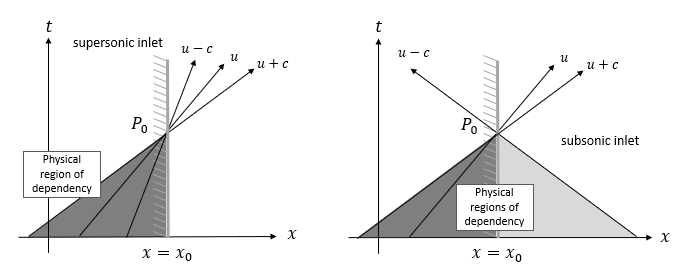
\includegraphics[height=6.0cm]{figs/boco_inlet_v2.png}
\caption{Boundary condition for one-dimensional inlet for Euler Equations with the internal (gray) and external (dark gray) physical regions of dependency \cite{Hirsch1991}.}
\label{fig:boco_inlet}
\end{figure}

Figure\ \ref{fig:boco_inlet} illustrates the $(x, t)$ plane around an arbitrary inlet point $P_0$ located at $x = x_0$ for the supersonic and subsonic cases. The former has all waves entering the domain once $u > c$ and consequently $u-c$ is positive. Therefore, the physical region of dependency propagates from the outside of the domain and, thus, all characteristics variables of $\textbf{W}$ must be given. On the other hand, for the subsonic inlet situation, the wave whose velocity is $u-c$ comes from the inside of the domain and, for this reason, it can not be known beforehand. For the subsonic case, only the characteristics related to $u$ and $u+c$ wave velocities must be imposed at the inlet boundary. The contributions associated with the wave with speed $u-c$ must be extrapolated from the inside. 

For supersonic inlet, the primitive properties associated with the characteristics variables for $u$,  $u-c$, and $u+c$ that are commonly chosen to be imposed are the free-stream pressure and velocity or an analytical solution when applied. Moreover, for the subsonic inlet, the velocity component is extrapolated from the interior domain.

\subsection{Outlet}
At an outlet boundary, analogously to the inlet boundary condition, the information dependency in the $(x, t)$ plane can also be illustrated. For the supersonic outlet, since all the region of dependency is inside of the domain, the properties must be extrapolated from the interior. On the other hand, for the subsonic outlet, commonly the static pressure is imposed due to the $u-c$ wave that is entering the domain and the other properties are extrapolated or calculated from the interior values.
%
\begin{figure}[htb!]
	\centering
		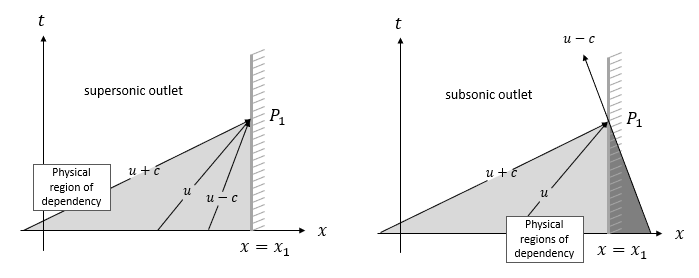
\includegraphics[height=6.0cm]{figs/boco_outlet_v2.png}
\caption{Boundary condition for one-dimensional outlet for Euler Equations with the internal (gray) and external (dark gray) physical regions of dependency \cite{Hirsch1991}.}
\label{fig:boco_outlet}
\end{figure}

\subsection{Non-Reflective Farfield}
By imposing values at the inlet and outlet when solving the Euler Equations, any wave that reaches these boundaries is reflected and stays inside the domain until the numerical dissipation damps its intensity. A simple solution is to expand the external boundary increasing the domain of the simulation so that the path where the wave propagates is sufficiently far that the numerical dissipation can indeed attenuate its magnitude before it arrives at the boundaries. Nonetheless, this methodology increases the computation cost once the simulation domain can become unfeasibly large. Another possible outcome for this problem is to properly impose the characteristics using the Riemann invariants approximating the 1D local solution for the characteristic problem normal to the boundary walls.

\section{Non-Dimensionalization}
%
The primitive properties of a fluid such as density, pressure and velocity can be represented in several different units and scales. For instance, a density field could range from $10^0-10^1 \frac{kg}{m^3}$ while a pressure field from $10^5-10^6 \frac{kg}{m.s^2}$, i.e., around 6 orders of magnitude higher than the density. From a numerical perspective, since only a discrete sample of real numbers can be processed in a computer, a wide numerical range of the properties in terms of the order of magnitude can cause high truncation errors and affect the numerical solution. Consequently, the numerical scale which a model is being iterated is relevant to the simulation output and for this purpose a non-dimensionalization procedure of the fluid properties is necessary. The most common approach is to determine beforehand reference values related to the application and then to rewrite the governing equations with the normalized properties defined as
%
\begin{align}
    \label{non_dim}
	\overline{t} &= \frac{t  c_{ref}}{L_{ref}} &
	\overline{L} &= \frac{L}{L_{ref}}
\end{align}
%
\begin{align}
    \label{non_dim2}
	\overline{\rho} &= \frac{\rho}{\rho_{ref}} &
	\overline{\textbf{U}} &= \frac{\textbf{U}}{c_{ref}} &
	\overline{p} &= \frac{p}{\rho_{ref} c^{2}_{ref}}
\end{align}
%
\begin{align}
    \label{non_dim3}
	\overline{E} &= \frac{E}{\rho_{ref} c^{2}_{ref}} &
	\overline{T} &= \frac{T}{T_{ref}  c^{2}_{ref}}
\end{align}
%
where $_{ref}$ subscripted properties represent reference values and in several applications they can refer to the free-stream reference values being subscripted by $_{\infty}$ symbol instead. The speed of sound, $c$, can be written in terms of the primitives over the assumption of calorically perfect gas using isentropic relations as
%
\begin{align}
    \label{sos}
    c &= \sqrt{\left(\frac{\partial p}{\partial \rho}\right)_{s}} = \sqrt{\frac{\gamma p}{\rho}} = \sqrt{\gamma R T}
\end{align}

